\documentclass[11pt,a4paper,oneside]{report}

\usepackage{amsmath}
\usepackage{graphicx}

\graphicspath{ {./images/} }

\begin{document}
	
\section{Vector diagram}

\begin{center}
	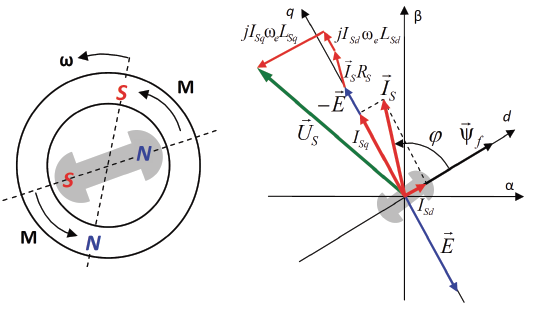
\includegraphics[scale=1]{motor}
\end{center}

Denote $\vec{\psi_f}$ rotor flux linkage. $\vec{\psi_f}$ lags behind $\vec{I_s}$ by an angle $\varphi$.

Rotor flux creates EMF in stator armature:

\begin{equation}
	E=\psi_f\omega_e,
\end{equation}
where $\omega_e=Z\omega_r$ is a pole angular velocity, $\omega_r$ is a rotor angular velocity, $Z$ is a number of pole pairs.

According to (ref{diagram})
\begin{equation}
	\vec{U_s} = -\vec{E}+\vec{I_s}R_s+j\omega_e(\vec{I_{sd}}L_{sd}+\vec{I_{sq}}L_{sq})
\end{equation}

For non-salient motor $L_{sd}=L_{sq}=L$.

\section{Momentum equation}

\begin{equation}
	M_e=Z(I_{sq}\psi_{sd}-I_{sd}\psi_{sq}) = Z(\psi_{s\alpha}i_{s\beta}-\psi_{s\beta}i_{s\alpha})
\end{equation}

\begin{equation}
	M_e=Z(I_{sq}\psi_f+I_{sd}I_{sq}(L_{sd}-L_{sq}))
\end{equation}

For non-salient motor
\begin{equation}
	M_e=Z(I_{sq}\psi_f)
\end{equation}

\section{Electric equations}

Stator equations
\begin{equation}
	\left\{
	\begin{split}
		U_{s\alpha} = \frac{d\psi_{s\alpha}}{dt}+R_sI_{s\alpha}\\
		U_{s\beta} = \frac{d\psi_{s\beta}}{dt}+R_sI_{s\beta}
	\end{split}
	\right.
\end{equation}

Consider flux linkage derivatives. There is no rotor flux changes along $d$-axis. Therefore
\begin{equation}
	\frac{d\psi_{sd}}{dt}=L_{sd}\frac{dI_{sd}}{dt}+f_d(\omega_e)
\end{equation}
where $f_d(\omega_e)$ is a term created by rotor rotation.

Flux derivative for $q$-axis:
\begin{equation}
	\frac{d\psi_{sq}}{dt}=L_{sq}\frac{dI_{sq}}{dt}+E++f_q(\omega_e)
\end{equation}

Derivative of vector that rotates with angular velocity $\omega_e$ is a vector with magnitude equal to linear velocity of rotation vector and orthogonal to its trajectory. Because of rotates coordinate frame angle between vector and its derivative if $-\pi/2$.

\begin{center}
	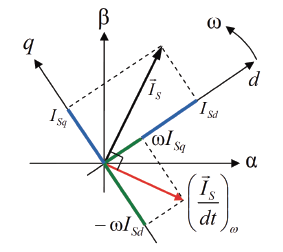
\includegraphics[scale=1]{vec_der}
\end{center}

Therefore
\begin{equation}
	\left\{
	\begin{split}
		f_d(\omega_e) = -\omega_eL_{sq}I_{sq}\\
		f_q(\omega_e) = \omega_eL_{sd}I_{sd}
	\end{split}
	\right.
\end{equation}

\section{Resulting equations}

\begin{equation}
	\left\{
	\begin{split}
		& pI_{sd}=\frac{1}{L_{sd}}(U_{sd}-R_sI_{sd}+\omega_eL_{sq}I_{sq})\\
		& pI_{sq} = \frac{1}{L_{sq}}(U_{sq}-R_sI_{sq}-\omega_eL_{sd}I_{sd}-\psi_f\omega_e)\\
		& M_e = Z(I_{sq}\psi_f+I_{sd}I_{sq}(L_{sd}-L_{sq}))
	\end{split}
	\right.
\end{equation}

Coordinates transformation:
\begin{equation}
	\begin{split}
		& U_{sd} = U_{s\beta}\sin\theta_e+U_{s\alpha}\cos\theta_e\\
		& U_{sq} = U_{s\beta}\cos\theta_e-U_{s\alpha}\sin\theta_e\\
		& I_{s\alpha} = I_{sd}\cos\theta_e-I_{sq}\sin\theta_e\\
		& I_{s\beta} = I_{sd}\sin\theta_e+I_{sq}\cos\theta_e
	\end{split}
\end{equation}

	
\end{document}